\section{Core Phase-1 results}

\subsection{Known-pose cooperative ranging corrects inertial drift}
Figure~\ref{fig:summary_p1a} shows the baseline behavior. With approximately known initial state, noisy inertial dead reckoning gradually drifts away from the reference trajectory, whereas the PF repeatedly uses UWB ranges to pull the position estimate back toward the truth. Across the 20-seed P1B baseline, mean position RMSE decreases from \(1.491\pm0.635\)~m for dead reckoning to \(0.375\pm0.196\)~m for PF+UWB, with lower position RMSE in all 20 seeds.

\begin{figure}[htbp]
    \centering
    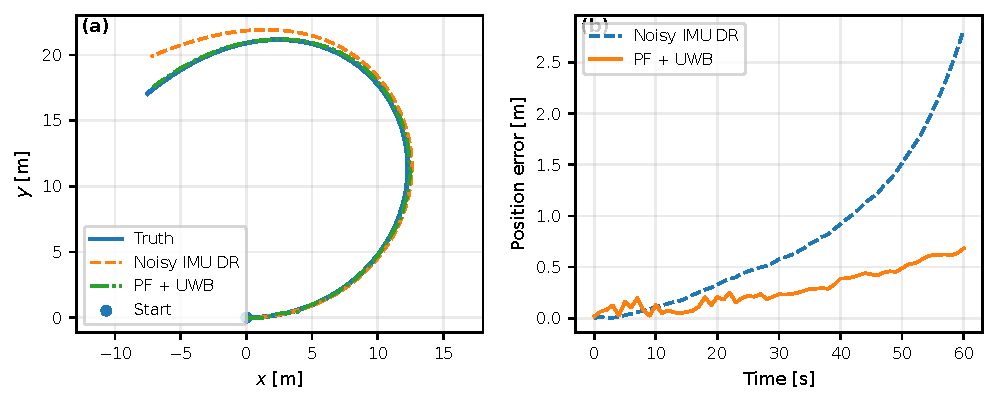
\includegraphics[width=0.94\textwidth]{figures/phase1/p1a_baseline_trajectory.pdf}
    \caption{Known-pose baseline: trajectory and position-error history for the representative P1A run.}
    \label{fig:summary_p1a}
\end{figure}

The result should be interpreted narrowly: UWB is demonstrably useful for position-drift correction in this controlled setting. The current scalar range measurement does not directly improve yaw, and large initial uncertainty or persistent IMU bias can still cause failure.

\subsection{Geometry is necessary, but not sufficient}
The unknown-pose problem exposes a more fundamental limitation. Figure~\ref{fig:summary_p1d} compares three auxiliary-node geometries. Stationary and constructed constant-bearing cases remain locally rank deficient, while an informative moving auxiliary eventually produces a full-rank finite-horizon linearized observability matrix.

\begin{figure}[htbp]
    \centering
    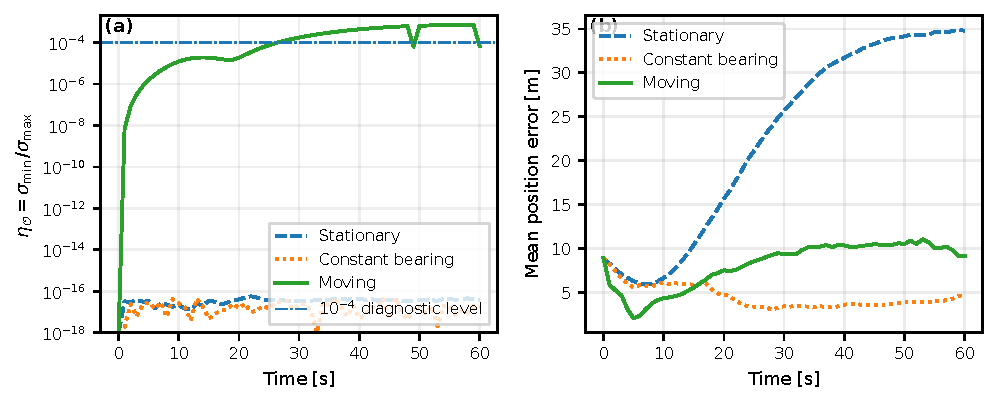
\includegraphics[width=0.94\textwidth]{figures/phase1/p1d_geometry_observability.pdf}
    \caption{Geometry and observability: normalized finite-horizon conditioning and mean position error for stationary, constant-bearing, and informative moving auxiliary trajectories.}
    \label{fig:summary_p1d}
\end{figure}

Only the moving case supports full-pose recovery, but realistic success is still limited. This establishes the key Phase-1 distinction:
\begin{equation}
    \boxed{\text{informative geometry is necessary but does not guarantee finite-particle acquisition.}}
\end{equation}

The paper-level conventional-PF study makes the support issue explicit. Figure~\ref{fig:summary_p1fa} shows that increasing particle count can improve performance, but not monotonically. At \(N_p=10{,}000\), every initial cloud contains particles in the diagnostic correct region, yet strict pose success is only \(4/20\). Even at \(40{,}000\) particles, success is \(9/20\).

\begin{figure}[htbp]
    \centering
    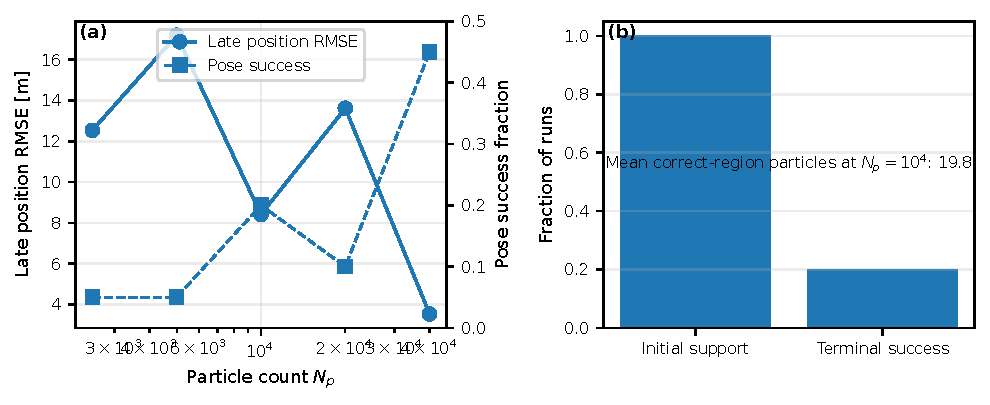
\includegraphics[width=0.94\textwidth]{figures/phase1/p1fa_global_pf_scaling.pdf}
    \caption{Paper-state global PF: particle-count sensitivity and the gap between initial correct-mode support and terminal strict pose success.}
    \label{fig:summary_p1fa}
\end{figure}

The practical problem is therefore not simply insufficient particle count. Useful hypotheses must also survive sequential weighting and mode selection.

\subsection{Literal AACOPF does not solve the acquisition problem}
The Han et al. AACOPF mechanism was audited and reproduced under explicit assumptions. Its literal all-pairs transition copies particles toward higher-weight destinations. In controlled bimodal experiments this can rapidly amplify the correct mode, but it can also collapse ancestry onto an early wrong mode.

After safety-aware tuning, the frozen tuple
\begin{equation}
    (\alpha,\beta,c_\lambda)=(0.5,0,2)
\end{equation}
achieves \(40/40\) correct-mode locks in the held-out controlled P1F-C study. That success does not transfer to sparse random-annulus global initialization. At \(N_p=1200\), P1F-D gives strict success \(2/20\) for conventional PF versus \(1/20\) for literal AACOPF. AACOPF often reduces late error, but this is an error-shaping effect rather than a global-convergence improvement.

The negative controls further constrain the claim. In stationary geometry, the paper-state problem has an exact rotational gauge; the PF can fit the measured ranges closely and become nearly point-concentrated while remaining globally wrong. No particle-transition rule can manufacture information that the geometry does not contain.

\subsection{Literal AACOPF is not inherently robust to bad UWB data}
P1F-F deliberately leaves the Gaussian likelihood unchanged while adding sparse gross errors, Gaussian-mixture contamination, and positive NLOS-like bursts. Figure~\ref{fig:summary_p1ff} shows that conventional PF retains higher correct-lock rates and lower wrong-lock rates across the tested stress families.

\begin{figure}[htbp]
    \centering
    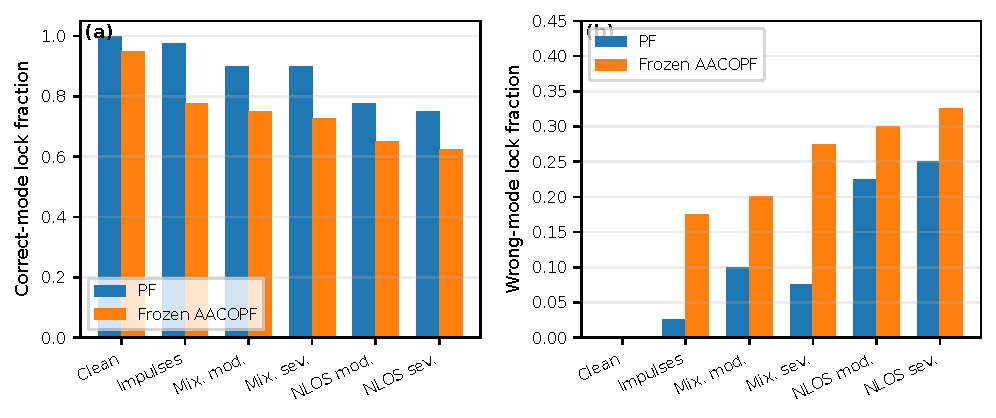
\includegraphics[width=0.94\textwidth]{figures/phase1/p1ff_ranging_stress.pdf}
    \caption{UWB ranging stress: correct- and wrong-mode lock fractions for conventional PF and frozen literal AACOPF.}
    \label{fig:summary_p1ff}
\end{figure}

Across the 200 stressed runs, conventional PF achieves \(86.0\%\) correct locks and \(13.5\%\) wrong locks; literal AACOPF achieves \(70.5\%\) correct locks and \(25.5\%\) wrong locks. Particle copying is therefore not a substitute for an explicit robust likelihood, gate, or reliability model.

\subsection{Guarded AACOPF fixes scaling and genealogy, not acquisition}
The final P1F-G adaptation bounds destination scoring to the top-\(K\) weighted candidates and introduces a move cap plus a per-destination incoming-copy capacity. The selected setting is
\begin{equation}
    K=8,\qquad
    f_{\mathrm{move}}=0.10,\qquad
    f_{\mathrm{dest}}=0.025.
\end{equation}

Figure~\ref{fig:summary_p1fg} summarizes the result. Candidate truncation alone is unsafe: it produces \(52.5\%\) wrong locks and catastrophic collapse in all held-out controlled runs. Adding the diversity guards restores \(40/40\) correct locks with no catastrophic collapse or dominant clone.

\begin{figure}[htbp]
    \centering
    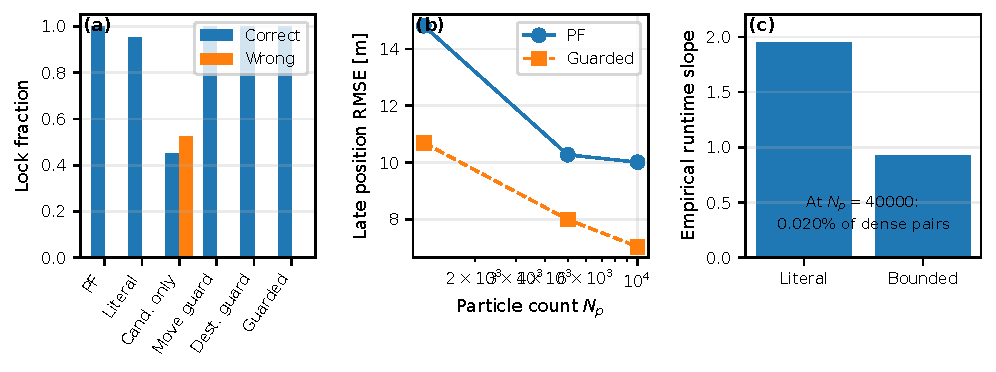
\includegraphics[width=0.98\textwidth]{figures/phase1/p1fg_scalable_guarded.pdf}
    \caption{P1F-G scalable guarded adaptation: controlled ablation, held-out global late-error comparison, and empirical runtime-scaling slopes.}
    \label{fig:summary_p1fg}
\end{figure}

The global result remains deliberately limited. Strict success for PF/guarded AACOPF is \(1/20\) vs.\ \(0/20\) at \(N_p=1200\), \(2/20\) vs.\ \(2/20\) at \(5000\), and \(3/20\) vs.\ \(1/20\) at \(10{,}000\). The guarded method does reduce mean late position and yaw RMSE at every evaluated population, but it does not solve broad-prior global acquisition.

Computationally, however, the adaptation is successful. The empirical runtime slope changes from approximately \(1.95\) for the literal reference to \(0.93\) for the bounded transition. At \(N_p=40{,}000\), only about \(0.020\%\) of the hypothetical dense pair count is scored.
